\documentclass{beamer}

\usetheme{Madrid}
\setbeamertemplate{footline}{}
\setbeamertemplate{navigation symbols}{}
\usepackage{graphicx}
\usepackage{tikz}
\usetikzlibrary{positioning,arrows.meta}
\title{Student Performance Analytics and Prediction}
\subtitle{SSL Project}
\author{
CS25BT029 \\
CS25BT042 \\
CS25BT052 }
\institute{\large Indian Institute of Technology Dharwad}
\date{November 16,2026}

\begin{document}

\begin{frame}
    \titlepage
\end{frame}

\begin{frame}{Problem Statement}
    Student marks and attendance contain useful information
    about academic performance. Analyzing this information
    manually can be time-consuming.

    \vspace{0.5cm}
    \textbf{Our solution:}
    \begin{itemize}
        \item Import student records using csv files.
        \item Analyze student marks and attendance systematically.
        \item Visualize subject-wise performance and overall performance.
        \item Predict average marks using Linear regression.
        \item Generate statistics such as total marks,average marks,grades and pass percentage.
    \end{itemize}
\end{frame}

\begin{frame}{Project Objectives}
    \begin{itemize}
        \item Validate and clean student performance data.
        \item Calculate subject-wise average marks.
        \item Identify overall student performance and pass percentage.
        \item Generate graphs to visualize performance trends and mark distributions.
        \item  Build and Evaluate a linear regression model to predict average marks.
        \item test the correctness and reliability of the implemented system.
    \end{itemize}
\end{frame}

\begin{frame}{Dataset}
    Our CSV dataset contains:
    \begin{itemize}
        \item Student ID
        \item Mathematics marks
        \item Physics marks
        \item Programming marks
        \item Attendance percentage
        \item Previous score
    \end{itemize}
\end{frame}

\begin{frame}{Methodology}
    \begin{enumerate}
        \item Collect student records in CSV format.
        \item clean missing and duplicate values.
        \item organise and prepare student records.
        \item Calculate statistics using Pandas.
        \item Generate graphs using Matplotlib.
        \item Train and evaluate a linear regression model.
        \item Test and profile the program.
        \item Predict final examination marks.
    \end{enumerate}
\end{frame}

\begin{frame}{Workflow}

\centering
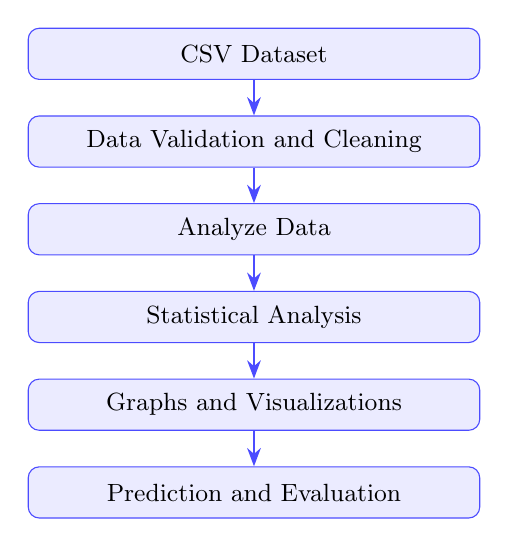
\begin{tikzpicture}[
    node distance=0.45cm,
    process/.style={
        rectangle,
        rounded corners=4pt,
        draw=blue!70,
        fill=blue!8,
        text width=5.5cm,
        minimum height=0.65cm,
        align=center,
        font=\small
    },
    arrow/.style={
        -{Stealth},
        thick,
        blue!70
    }
]

\node[process] (data) {CSV Dataset };
\node[process, below=of data] (clean) { Data Validation and Cleaning};
\node[process, below=of clean] (analysis) { Analyze Data};
\node[process, below=of analysis] (visual) {Statistical Analysis};
\node[process, below=of visual] (model) {Graphs and Visualizations};
\node[process, below=of model] (result) {Prediction and Evaluation};

\draw[arrow] (data) -- (clean);
\draw[arrow] (clean) -- (analysis);
\draw[arrow] (analysis) -- (visual);
\draw[arrow] (visual) -- (model);
\draw[arrow] (model) -- (result);

\end{tikzpicture}

\end{frame}

\begin{frame}{Tools and Technologies}
    \begin{itemize}
        \item Python - Programming language
        \item Pandas - data processing and analysis
        \item Matplotlib - Graphs and visualizations
        \item Scikit-learn - Linear regression and model evaluation
        \item CSV - dataset format
        \item Git \& GitHub - version control and project hosting
        \item Bash scripting - Automating project tasks
        \item LaTeX \& Beamer - report and presentation 
    \end{itemize}
\end{frame}

\begin{frame}{Results}
    \begin{itemize}
        \item Successfully imported and processed student data.
        \item Subject-wise averages are calculated.
        \item Student academic performance is visualized.
        \item A prediction model estimates average marks.
        \item Generated analytical reports.
        \item Functional tests check data validity.
    \end{itemize}

    \vspace{0.3cm}
\end{frame}
\begin{frame}{Average Marks by Subject}
    \centering
    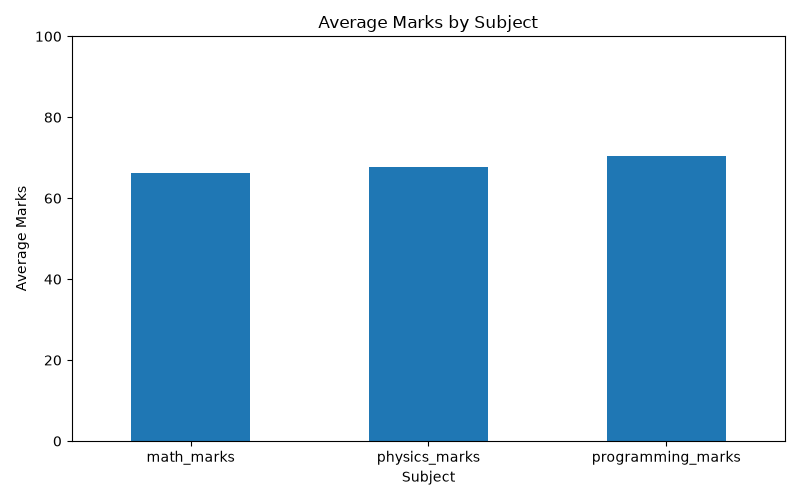
\includegraphics[width=0.85\textwidth]
    {subject_averages.png}
\end{frame}

\begin{frame}{Distribution of Student Average Marks}
    \centering
    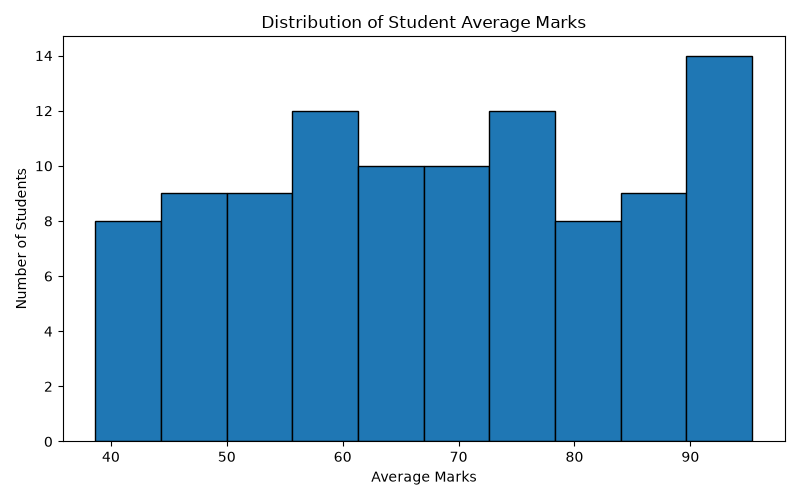
\includegraphics[width=0.85\textwidth]
    {avg_distribution.png}
\end{frame}

\begin{frame}{Conclusion}
    \textbf{Conclusion}
    \begin{itemize}
        \item The system automates basic student performance analysis.
        \item Provides visual insights and estimated average marks.
        \item Graphs make the results easier to understand.
        \item Supports better data-driven decisions.
    \end{itemize}
\end{frame}

\begin{frame}
    \centering
    \Huge Thank You!
    
    \vspace{0.5cm}
    
\end{frame}

\end{document}